\documentclass[12pt]{article}
\usepackage[margin=.25in]{geometry}
\usepackage{textcomp}
\usepackage{float, graphicx, color, soul}
\usepackage{amsmath}
\usepackage{listings}
\lstset{
basicstyle=\ttfamily,
frame=single,
numbers=left
}
\title{CS185C: \\ 
Final Exam Notes}
\author{Brett Dispoto}

\begin{document}
\maketitle

\section{Ensemble Learners}
An ensemble learner is defined as:

\begin{equation}
  F(x) = <\text{aggegrate function}>(\text{scoring functions...})
\end{equation}

\subsection{Scoring Function}
Where the scoring function is:
\begin{equation}
  S(x, V, \Lambda)
\end{equation}

Where...
\begin{enumerate}
  \item $x$ is the sample we wish to classify,
  \item $V$ is the training data,
  \item $\Lambda$ is a set of function parameters for the model. (initial weights, training param/hyperparam, etc)
\end{enumerate}


\subsection{Bagging}
Also called \textbf{bootstrap aggegration}, bagging is where \textit{different subsets of the data or features (or both)} are used to generate different scores.
\begin{enumerate}
  \item The results are then combined in some way, such as sum, average, or max.
  \item For bagging we assume that the same scoring model is used for all scores in the ensenble. 
  \item Bagging is meant to reduce overfitting.
  \item Very similar to n-fold validation.
  \item Good for small datasets, so we don't overfit on the data. 10 "bags" is probably a good initial choice.
  \item If the aggregate function we use is average, then we're actual just doing n-fold validation. 
  \item However, we can still apply n-fold validation ON TOP OF bagging. (In fact, we should if possible).
\end{enumerate}
For bagging the ensemble equation is:

\begin{equation}
  F(S(x, V_1, \Lambda), S(x, V_2, \Lambda), ... , S(x, V_l, \Lambda),
\end{equation}
Note that $\Lambda$ remains constant across all of our scoring fucntions. However, $V_i$ is changing to specify that we are using differnt parts of the dataset.
If we want to use diffent features... here's an exmaple for one of our models:


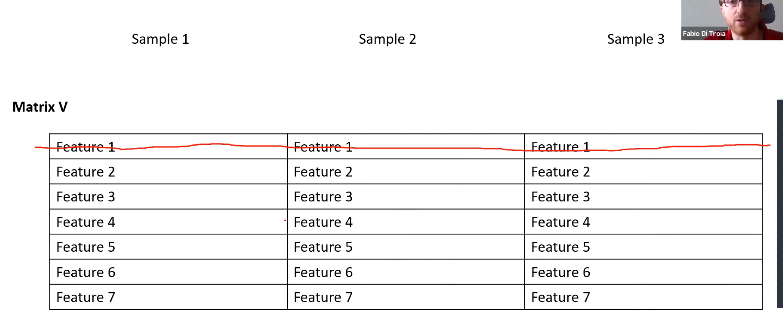
\includegraphics[width=.8\textwidth]{diffFeatures.png}
If we want to use different samples... here's an exmaple for one of our models:


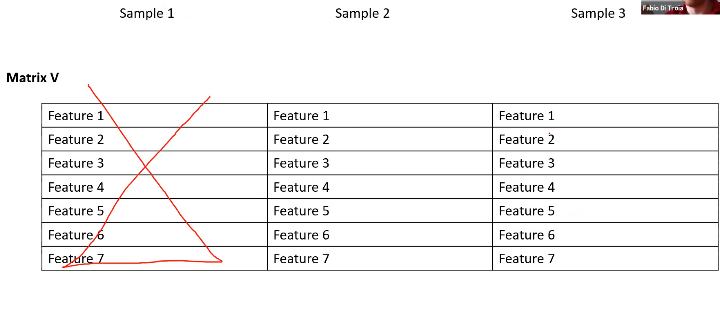
\includegraphics[width=.8\textwidth]{diffSamples.png}

More on bagging:
\begin{enumerate}
  \item How to choose feature selection? Experiments.
  \item We can also do subsets of both features and samples for a particular model.
  \item This kind of bagging works well for \textbf{random forrests}.
  \item \hl{We have to do an ensemble learner for \textbf{EACH} of the malware families.} For example, for the \textsc{WinWebSec} malware family, we have multiple \textsc{WinWebSec} HMMs, which will be used in conjunctin to create the \textsc{WinWebSec-Classifier}, which is our "ensembled" \textsc{WinWebSec} HMMs.
  \item \hl{For the this class, we should \textbf{NOT} split by features.} It may require too much domain knowledge. \hl{Also, there aren't really enough features to do this anyway.}
\end{enumerate}

\subsection{Boosting}
Boosting is where we only differ the model, and not the data. We usually use "weak" classifiers. However, for our class, we only care about boosting \textit{where the classifiers only differ in terms of their parameters} (So, we're not combining different types of models such as GAN, SVM, and HMM.

\textbf{Voting} workes better with boosting than with stacking. However, Fabio still recommends average or max in general. 

We can also do random restarts, where we select the best model, then combine the  results. HMM with random restarts can be seen as a special case of boosting, where we just pick the max.
\subsection{Stacking}

We can also use SVM as a meta-classifier, such that we no longer use of these aggegrate functions (max, average, etc..).



\section{Steps for Final}
Here are the steps to complete for the final. Crossed out means that it's finished.
\begin{enumerate}
  \item \st{Make an HMM.}
  \item Download the dataset.
  \item Add dataset to .gitignore
  \item Split the dataset into different directories based on the malware family they belong to.
  \item Do bagging. Create a file \texttt{Bagging.java}. Allow for command line arguments. The usage should be something like: 
        
    \texttt{java Bagging $<$file\_name$>$}

    where $<$file\_name$>$ is the name of the file we wish to classify.

  \item Here is what Bagging.java should do if passed the command line argument "train":
    \begin{enumerate}
      \item Train $n$ HMM's for \textit{each} malware familty. Save the HMMs into directories called \texttt{\$FAMILY.hmms/}.
      \item Save the HMM's to a file on disk, so they can be reloaded for classiflying.
    \end{enumerate}

  \item Here is what Bagging.java should do if passed a command line argument of a filename to classify.
    \begin{enumerate}
      \item For each malware family:
        \begin{enumerate}
      \item Load the HMM's from the file,
      \item Score the sample with each HMM,
      \item Use some aggregate function (max, sum, average, etc..).
      \item Write down the score for this malware family.
        \end{enumerate}
      \item Finally, compare all of the scores and pick the highest. The group of HMM'swhich produced the highest score gives us the malware family this sample has been classified as.
    \end{enumerate}
\end{enumerate}
\end{document}
